\subsection{Construction Activities }
\auth{
T.\,H.~Burritt, 
M.~Buuck,
C.~Cuesta,
J.\,A.~Detwiler,
J.~Gruszko,
\underline{I.~Guinn},
J.~Leon,
D.\,A.~Peterson,
R.\,G.\,H.~Robertson,
and
T.\,D.~Van~Wechel
}



\noindent     % This prevents the indentation of the first paragraph. Don't skip the next line.
The CENPA \MJ~group has been heavily involved in the construction of the \MJ~\MJDemo. In particular, CENPA students and staff have led the development and assembly of low background cable connectors for the \MJDemo. These connectors are used on the signal cables which run from the HPGe detector array to an electronic feedthrough flange outside of the shielding. Because of their close proximity to the detectors, a novel, spring-free design was necessary to ensure that backgrounds are low enough to meet the goals of the \MJDemo. Over the last year, 90 cables with female connectors were assembled and tested at UW with two main updates to their design. First, the dimensions of the connectors were tweaked to improve the reliability of their fit to male connectors. Second, the other end of the cables were soldered to 50-pin d-sub feedthrough flange connectors to reduce the risk of damaging cables during installation. These connectors are currently in use in both modules 1 and 2.

\begin{figure}[h]
  \hfil  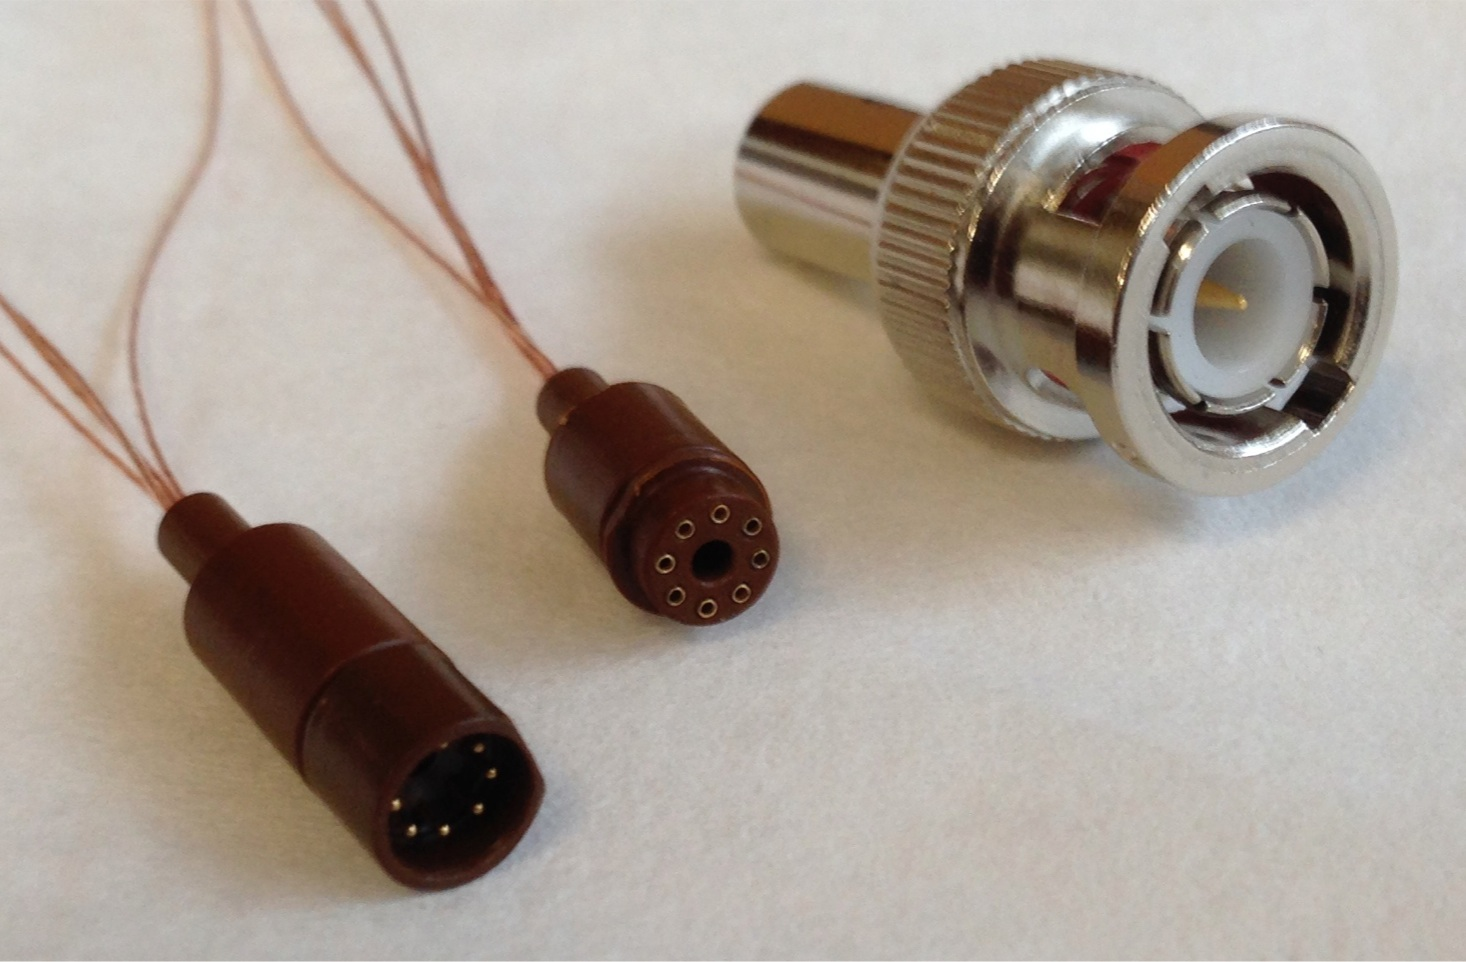
\includegraphics[width=.5\textwidth]{SigConBNCComparison.jpg} \hfil 
  \hfil  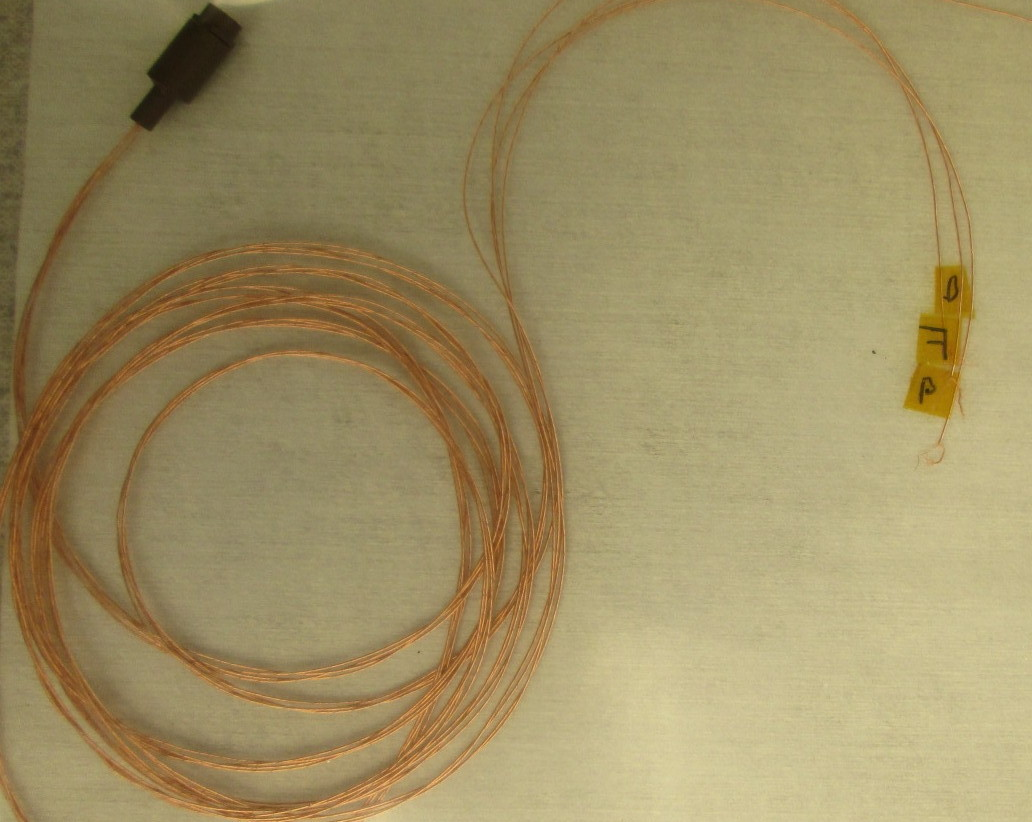
\includegraphics[width=.415\textwidth]{signal_bundle.JPG} \hfil 
  % the following blank line is important
  
  
  \figcaption{MJConnArticle}{{\it Left:} A signal plug pair, with a BNC connector for comparison. {\it Right:} A signal cable soldered to a signal plug.}
  
  \label{MJConnectors}  %put label{} after \figcaption{}
  
\end{figure}

CENPA collaborators have also been heavily involved in construction and operation of the experiment at SURF, enabling the \MJ~\MJDemo to reach several important milestones. Module 1 was installed and operated in-shield in May 2015. In October 2015, Module 1 was removed in order to make several design improvements. These improvements included the replacement of old signal cables with the updated design mentioned in the previous paragraph. In addition, the inner electroformed copper shield was installed along with additional shielding in the cryostat crossarm. Module 1 was reinstalled in shield in December 2015, and is currently in operation.
  
\begin{figure}[h]
\hfil  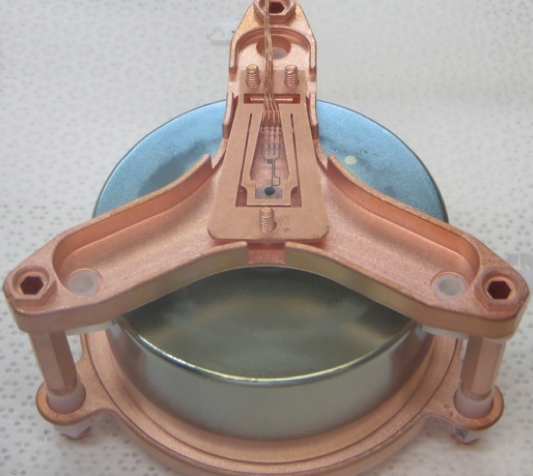
\includegraphics[width=.60\textwidth]{MJD_detectorUnit.png} \hfil 
\hfil  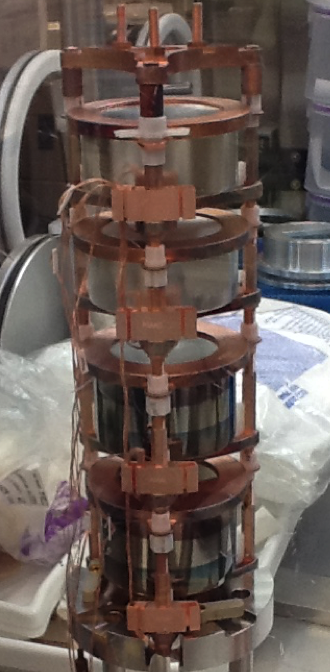
\includegraphics[width=.30\textwidth]{MJD_string.png} \hfil
% the following blank line is important

~

\figcaption{StringBuilding}{{\it Left:} The \MJ~detector unit holds a P-type point contact HPGe detector and low-mass front end. {\it Right:} Detector assemblies are stacked to create a string.}

\label{MJD_Assemblies}  %put label{} after \figcaption{}

\end{figure}


Construction of Module 2 is also well underway. All seven strings of detectors for Module 2 have been assembled. The assembly process was improved over Module 1's by the implementation of a modernized quality control procedure using the elog system, developed by Julieta Gruszko. In addition, the cryostat and vacuum hardware for Module 2 have been assembled and commissioned. The strings will be loaded into the cryostat by the end of April 2016, and commissioning of the detectors will begin soon after.

\begin{figure}[h]

\hfil  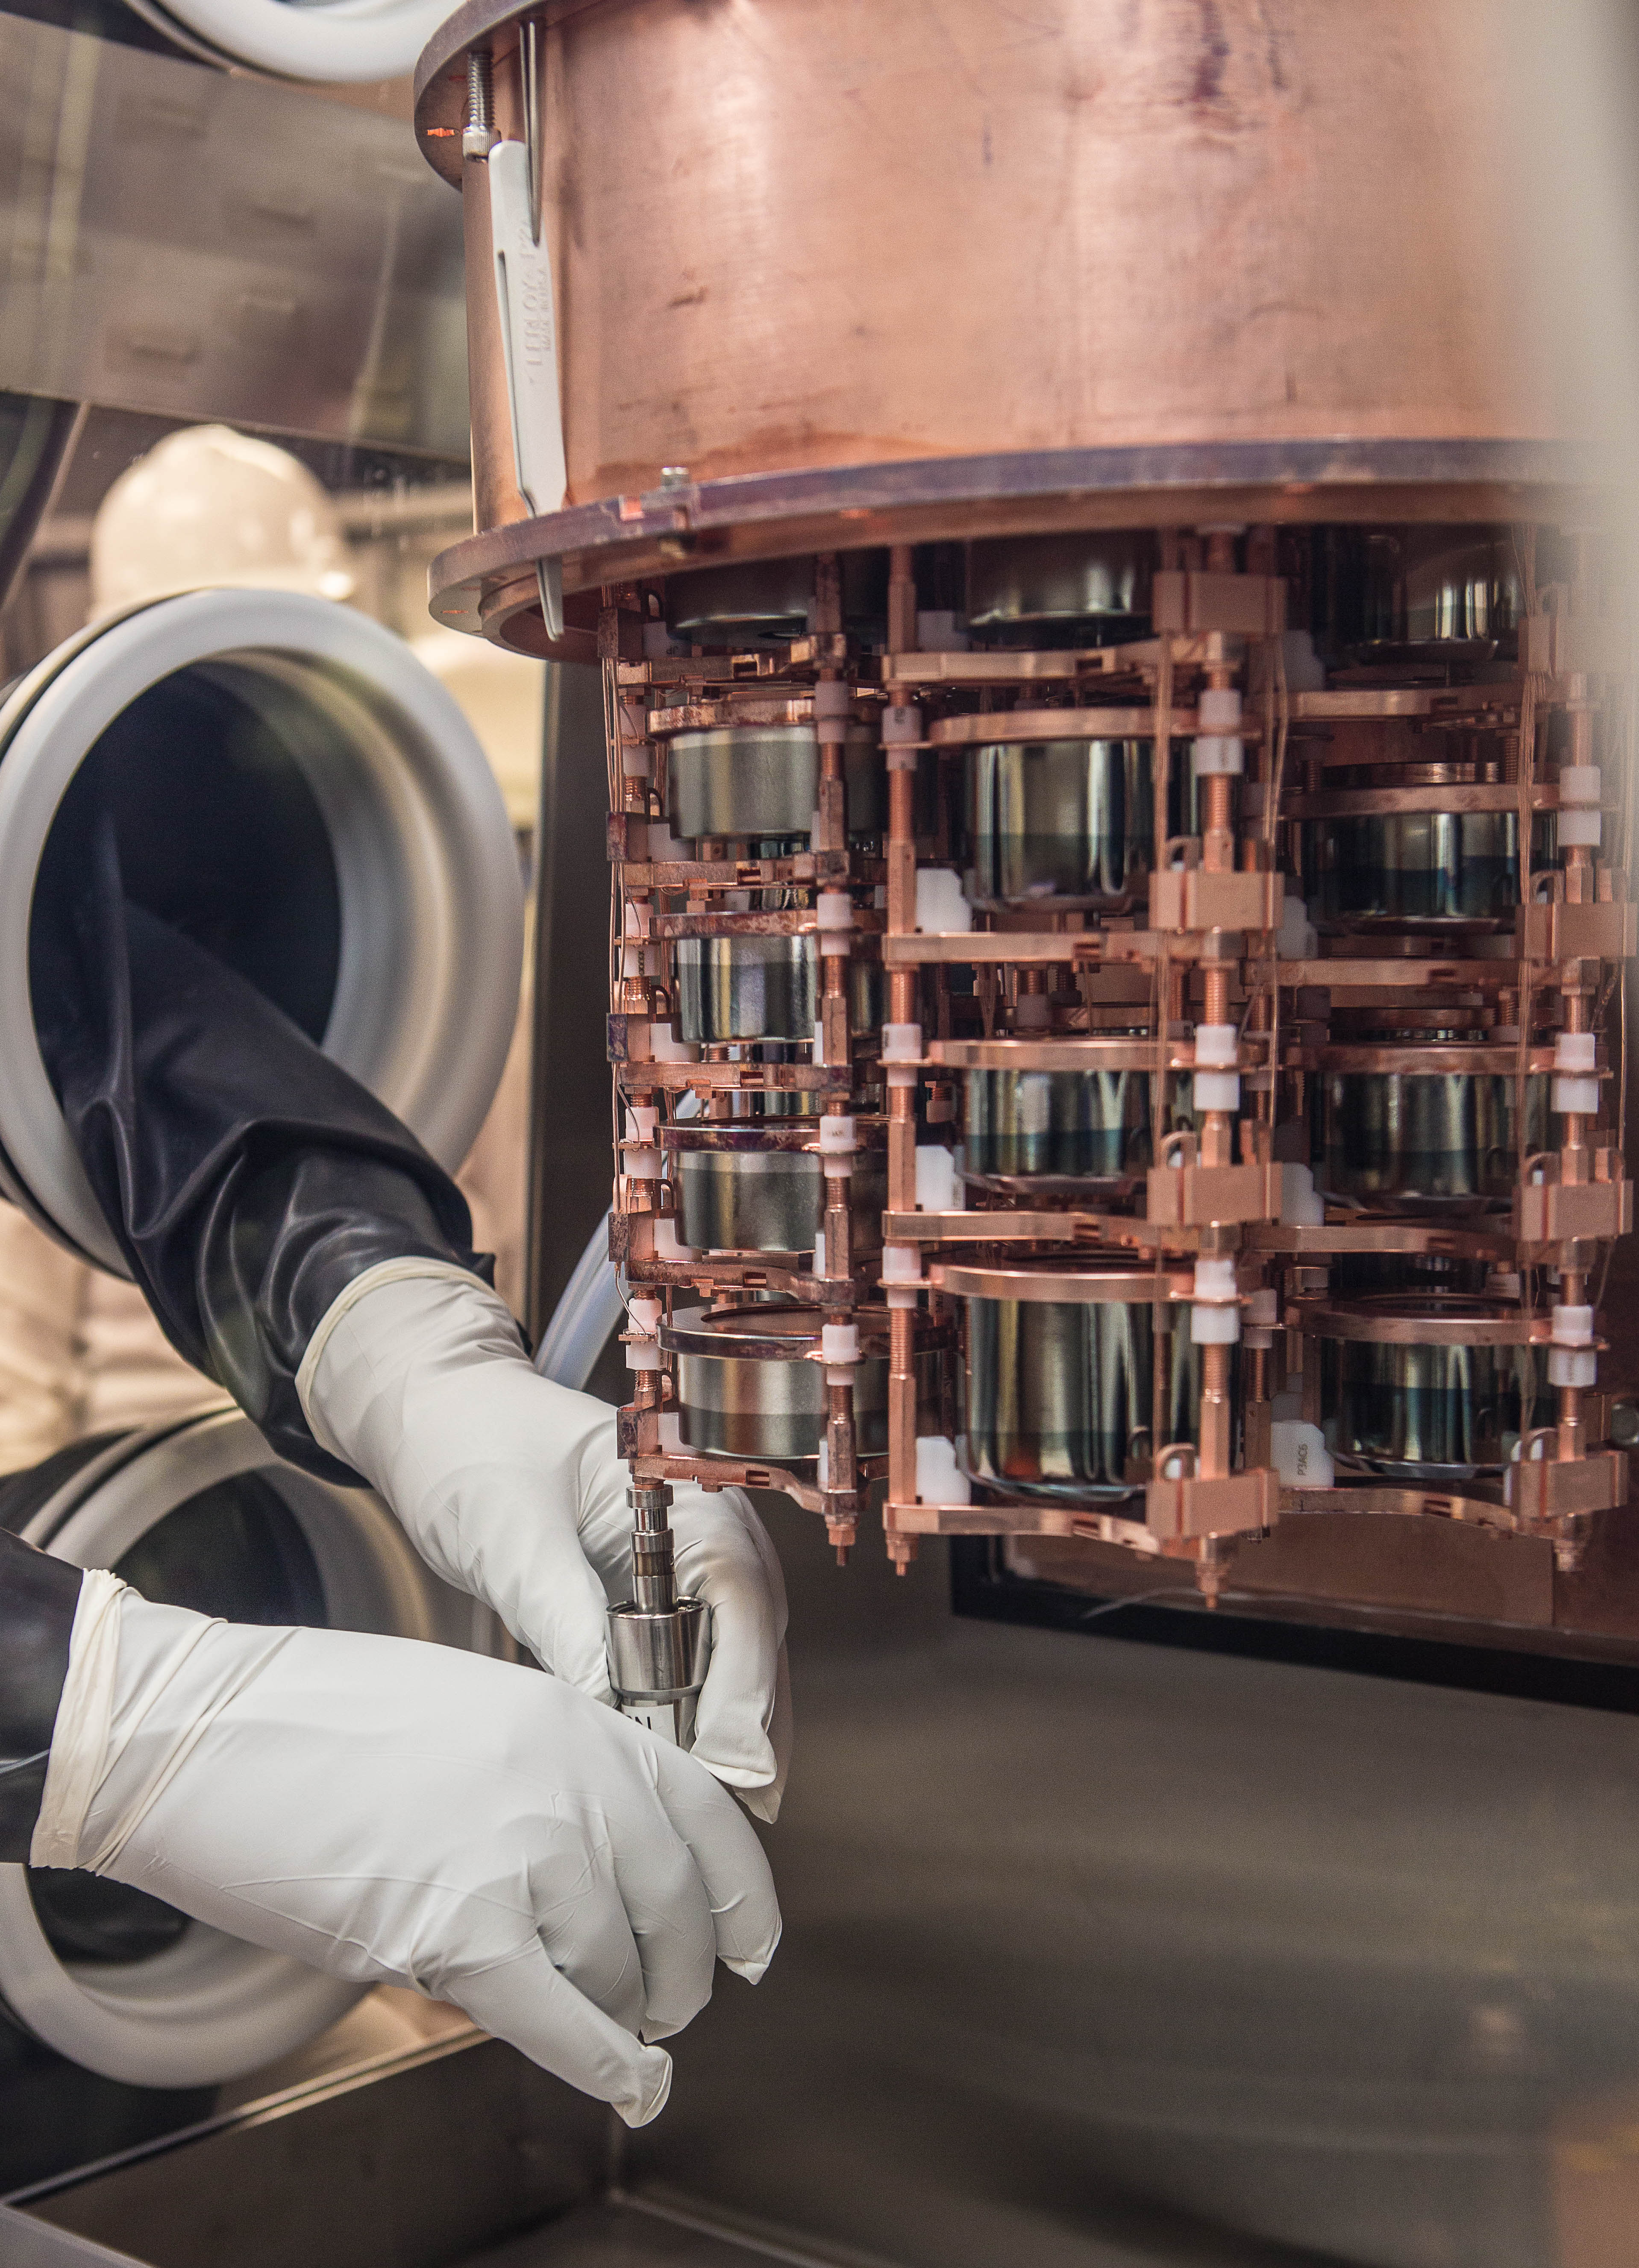
\includegraphics[width=.45\textwidth]{MJD_StringInstall.jpg} \hfil 
% the following blank line is important

\figcaption{StringBuilding}{Seven strings are installed in each module of the \MJ~\MJDemo.}

\label{MJD_StringInstall}  %put label{} after \figcaption{}

\end{figure}
